% 图 24.4 —— 由 `checks/emit_hand.py` 自动拼出（probe 精测 + prims2 图元分解）
%%
% ⚠ 这是**稿子不是成品**：跑 `checks/checkhand.py 24.4` 看指标 + 看叠合图。
%%
%% ⚠ 待核：
%   · 本图 probe 报出阴影族 1 个 —— **本脚本不生成阴影**（要照原书手写）；prims2 的 strokes 里可能含阴影线，核对时留意别画重
%   · 可疑字形 1 项（空心圈 ⊙ 常被认成字母 o）—— 见文件末
%%
\documentclass[12pt]{standalone}
\usepackage{fontspec}
\setsansfont{Arial}
\newfontfamily\mfallback{DejaVu Sans}
\usepackage{tikz}
\usetikzlibrary{arrows.meta}
\begin{document}
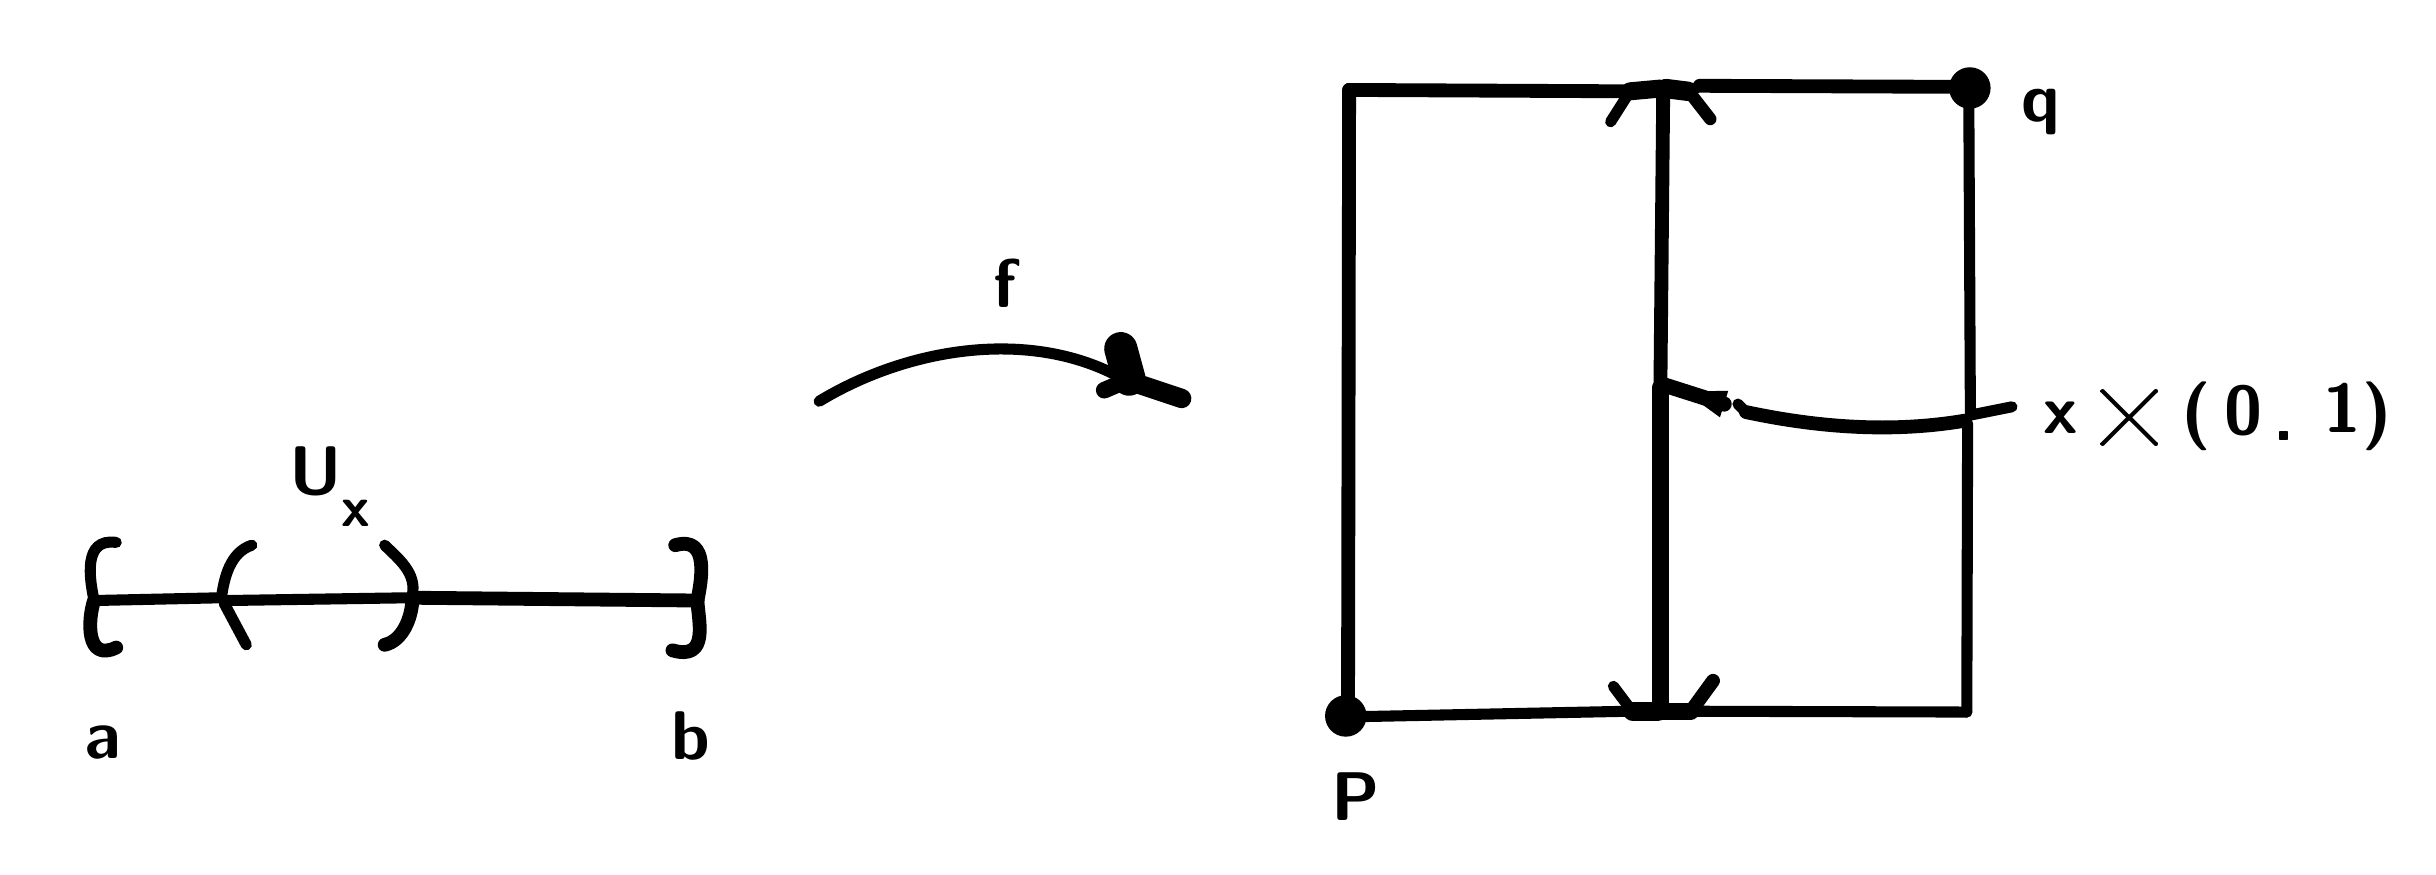
\begin{tikzpicture}[x=1pt, y=-1pt, line width=4.0pt, line cap=round, line join=round]

  %% ════ 填充区（prims2 的 fills）════

  %% ════ 直线段（prims2 的 strokes）════
  \draw[line width=4.0pt] (71.0,208.0) -- (79.0,223.0);
  \draw[line width=4.0pt] (702.0,140.0) -- (701.4,21.4);
  \draw[line width=5.0pt] (701.4,21.4) -- (604.2,21.0);
  \draw[line width=3.8pt] (604.2,21.0) -- (601.0,23.0);
  \draw[line width=4.0pt] (702.0,140.0) -- (717.0,137.0);
  \draw[line width=4.0pt] (72.0,207.0) -- (138.0,206.0);
  % （略）线段 (617.0,148.0)-(614.0,137.0) 线宽7.0 —— 是箭头头那一坨，已由箭头头代替
  \draw[line width=4.0pt] (70.0,206.0) -- (24.0,207.0);
  \draw[line width=5.0pt] (140.0,206.0) -- (242.0,207.0);
  \draw[line width=5.0pt] (590.0,128.0) -- (591.0,23.0);
  \draw[line width=4.0pt] (579.0,246.0) -- (573.0,238.0);
  \draw[line width=6.5pt] (590.0,22.0) -- (579.0,23.0);
  \draw[line width=7.0pt] (417.0,134.0) -- (399.0,128.0);
  \draw[line width=4.0pt] (618.0,136.0) -- (620.9,138.9);
  \draw[line width=5.5pt] (591.0,129.0) -- (613.0,136.0);
  \fill (614.5,131.2) -- (611.5,140.8) -- (598.7,131.5) -- cycle;
  \draw[line width=6.0pt] (590.0,130.0) -- (590.0,246.0);
  \draw[line width=7.0pt] (580.0,247.0) -- (589.0,247.0);
  \draw[line width=4.5pt] (608.0,33.0) -- (601.0,24.0);
  \draw[line width=5.0pt] (579.0,23.0) -- (477.5,22.5);
  \draw[line width=5.0pt] (477.5,22.5) -- (477.1,247.1);
  \draw[line width=2.9pt] (477.1,247.1) -- (479.3,249.0);
  \draw[line width=4.0pt] (479.3,249.0) -- (579.0,247.0);
  \draw[line width=4.0pt] (579.0,23.0) -- (572.0,34.0);
  \draw[line width=5.0pt] (601.0,247.0) -- (609.0,236.0);
  \draw[line width=6.0pt] (601.0,247.0) -- (591.0,247.0);
  \draw[line width=4.0pt] (601.0,247.0) -- (700.7,247.3);
  \draw[line width=4.0pt] (700.7,247.3) -- (701.0,143.0);
  \draw[line width=12.0pt] (395.0,116.0) -- (398.0,127.0);
  \draw[line width=7.0pt] (592.0,22.0) -- (600.0,23.0);
  \draw[line width=6.0pt] (389.0,131.0) -- (396.0,128.0);
  % （略）线段 (623.0,132.0)-(618.0,135.0) 线宽6.2 —— 是箭头头那一坨，已由箭头头代替

  %% ════ 曲线（prims2 的 curves —— 三段式，坐标同为 (y,x)）════
  \draw[line width=5.0pt] (139.0,207.0) .. controls (138.7,213.1) and (135.6,221.5) .. (129.0,223.0);
  \draw[line width=5.0pt] (234.0,187.0) .. controls (246.6,183.4) and (243.4,200.0) .. (242.0,207.0);
  \draw[line width=4.0pt] (70.0,206.0) .. controls (71.0,198.8) and (73.1,189.6) .. (81.0,187.0);
  \draw[line width=5.0pt] (233.0,225.0) .. controls (246.5,228.9) and (242.3,214.0) .. (242.0,207.0);
  \draw[line width=4.0pt] (139.0,205.0) .. controls (140.6,197.1) and (134.1,192.0) .. (129.0,187.0);
  \draw[line width=4.0pt] (396.0,127.0) .. controls (362.5,108.1) and (317.8,115.7) .. (286.0,135.0);
  \draw[line width=5.0pt] (620.9,138.9) .. controls (646.7,144.4) and (673.5,146.5) .. (700.0,142.0);
  \draw[line width=5.0pt] (32.0,224.0) .. controls (20.8,229.4) and (21.8,213.6) .. (24.0,207.0);
  \draw[line width=4.0pt] (32.0,186.0) .. controls (19.8,184.3) and (22.4,199.3) .. (24.0,207.0);

  %% ════ 实心点 ════
  \fill (701.8,21.8) circle (7.5);
  \fill (476.3,248.7) circle (7.5);

  %% ════ 标签（probe 直接给的 \node 行）════
  %% ⚠ 全部补了 fill=white：文字在最上层，否则与曲线交叉干扰
     \node[anchor=center,inner sep=0pt,fill=white,font=\fontsize{30.5}{38.1}\selectfont] at (727.5,30.8) {\textsf{\textbf{\textit{q}}}};   % box(718,18,17,22)
     \node[anchor=center,inner sep=0pt,fill=white,font=\fontsize{28.5}{35.6}\selectfont] at (354.0,92.5) {\textsf{\textbf{\textit{f}}}};   % box(348,81,11,22)
     \node[anchor=center,inner sep=0pt,fill=white,font=\fontsize{30.7}{38.4}\selectfont] at (783.5,140.5) {\textsf{\textbf{(}}};   % box(779,126,8,28)
     \node[anchor=center,inner sep=0pt,fill=white,font=\fontsize{32.7}{40.8}\selectfont] at (836.3,137.5) {\textsf{\textbf{1}}};   % box(827,126,11,22)
     \node[anchor=center,inner sep=0pt,fill=white,font=\fontsize{32.6}{40.7}\selectfont] at (849.1,140.5) {\textsf{\textbf{)}}};   % box(843,126,9,28)
     \node[anchor=center,inner sep=0pt,fill=white,font=\fontsize{30.6}{38.2}\selectfont] at (800.5,138.3) {\textsf{\textbf{0}}};   % box(791,127,14,22)
     \node[anchor=center,inner sep=0pt,fill=white,font=\fontsize{29.1}{36.4}\selectfont] at (734.5,140.9) {\textsf{\textbf{\textit{x}}}};   % box(726,130,15,18)
     \node[anchor=center,inner sep=0pt,fill=white,font=\fontsize{33.8}{42.3}\selectfont] at (759.6,141.0) {\textsf{\textbf{×}}};   % box(751,131,16,15)
     \node[anchor=center,inner sep=0pt,fill=white,font=\fontsize{53.0}{66.3}\selectfont] at (815.5,147.4) {\textsf{\textbf{.}}};   % box(809,142,5,10)
     \node[anchor=center,inner sep=0pt,fill=white,font=\fontsize{29.6}{37.0}\selectfont] at (104.0,160.2) {\textsf{\textbf{\textit{U}}}};   % box(94,148,20,22)
     \node[anchor=center,inner sep=0pt,fill=white,font=\fontsize{21.3}{26.6}\selectfont] at (118.7,175.4) {\textsf{\textbf{\textit{x}}}};   % box(112,168,12,12)
     \node[anchor=center,inner sep=0pt,fill=white,font=\fontsize{30.7}{38.3}\selectfont] at (239.8,255.8) {\textsf{\textbf{\textit{b}}}};   % box(230,243,17,23)
     \node[anchor=center,inner sep=0pt,fill=white,font=\fontsize{30.0}{37.6}\selectfont] at (27.5,258.5) {\textsf{\textbf{\textit{a}}}};   % box(19,249,15,16)
     \node[anchor=center,inner sep=0pt,fill=white,font=\fontsize{29.2}{36.4}\selectfont] at (479.9,278.0) {\textsf{\textbf{\textit{P}}}};   % box(469,266,18,22)

  % 钉死画布：否则超出的图元/控制点会把页面撑大，1:1 回比就失准
  \pgfresetboundingbox
  \path[use as bounding box] (0,0) rectangle (860,296);
\end{tikzpicture}
\end{document}

% ⚠ 待核清单（probe 拿不准，人眼过一遍）：
%   · 未识别/跳过：⑤ 跳过/未识别的字形
